\documentclass{article}
\usepackage{graphicx}
\usepackage{float}
\usepackage{amsmath}
\usepackage{amssymb}
\usepackage{amsfonts}
\usepackage{hyperref}
\usepackage{xcolor}
\usepackage{todonotes}
\usepackage{subfig}
\usepackage{caption}
\usepackage[ruled]{algorithm2e}

\newcommand{\D}{\mathbf{D}}
\newcommand{\Q}{\mathbf{Q}}
\DeclareMathOperator{\tr}{tr}
\title{Face Image Fitting and Its Applications\footnote{This is the first time we try to write the course project report in English. Your understanding is much appreciated.}}
\author{Kangcheng Hou\footnote{kangchenghou@gmail.com} \and Shuqi Wang\footnote{shuqiwang.cn@gmail.com} \and Tianhao Wei \footnote{phi.wth@gmail.com}}
\date{\today}
 

\newcommand{\pic}[2] {
    \begin{figure}[H]
    \centering
    \includegraphics[width=.6\textwidth]{./img/#1}
    \caption{#2}
    \end{figure}
}

\DeclareMathOperator*{\argmax}{arg\,max}
\DeclareMathOperator*{\argmin}{arg\,min}

\begin{document}

\maketitle
\tableofcontents

\section{Introduction}
A large proportion of images people uploaded is facial images. Motivated by this, in this course project, we want to develop a software that ease the process of editing facial image. The core part of our course project is face fitting, i.e. given a image, find the corresponding 3D model of the image. We also build two applications based upon the face fitting module.

The first one is to substitute the mouth in one image to another. The second one is to provide accessible way to edit face.
\begin{figure}
    \centering
    \subfloat[]{\includegraphics[width=0.4\textwidth]{./img/app11}}
    \hfill
    \subfloat[]{\includegraphics[width=0.4\textwidth]{./img/app12}}
    \caption{One application of face fitting is to transfer the smile from face (a) to face (b)}
\end{figure}
\begin{figure}
    \centering
    \subfloat[]{\includegraphics[width=0.4\textwidth]{./img/app21}}
    \hfill
    \subfloat[]{\includegraphics[width=0.4\textwidth]{./img/app22}}
    \caption{Another application of face fitting is to easily manipulate the face image without much artifact.}
\end{figure}

\subsection{Structure of the report}
In this report, we will first introduce the core part of this project, i.e. to reconstruct the 3D face model from a single image. Then we will introduce pipelines of two applications and their underlying techniques. Lastly, we will have a summary.
      

\section{Model fitting}
\subsection{Introduction}
Given a photo, we want to find a facial model fitted to the image. The typical method previously used is to first find the 2d feature points of the face and fit the 3d model to the image.

\begin{figure}[H]
\minipage{0.33\textwidth}
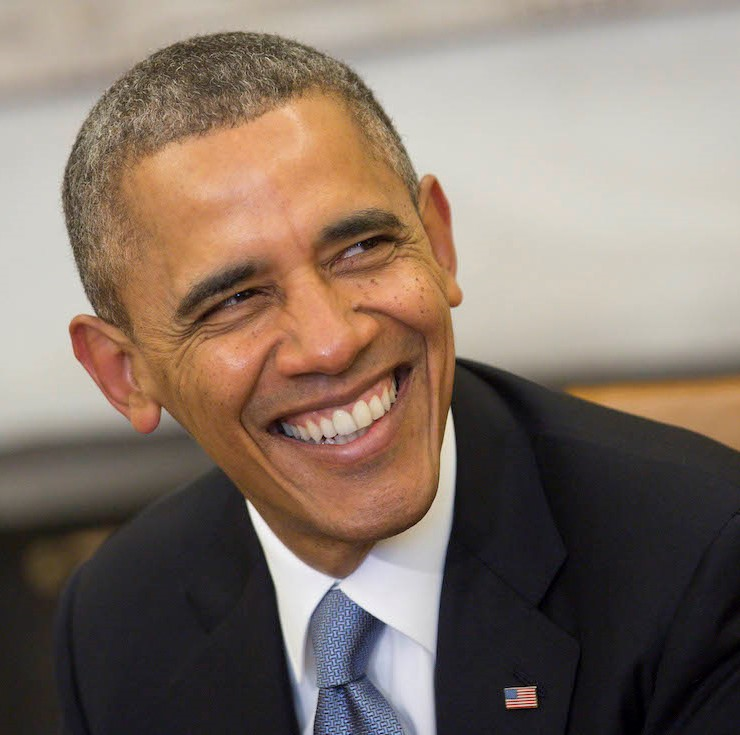
\includegraphics[width=\linewidth]{./img/img}
\endminipage\hfill
\minipage{0.33\textwidth}
\includegraphics[width=\linewidth]{./img/img_lm}
\endminipage\hfill
\minipage{0.33\textwidth}
\includegraphics[width=\linewidth]{./img/img_model}
\endminipage
\caption{The image, feature points and the fitted model}
\end{figure}
We first use state-of-the-art commercial software provided by face++\footnote{https://www.faceplusplus.com.cn/} to track the feature points $L^{(1), \cdots, (K)}$ which can be seen from the figure. Note that we include the points on the contour. As we will see later, feature points on the contour will be very helpful for fitting the model. Then we will fit a 3D model based on these points.

\subsection{Parametric Face Model}
Parametric face model use a low dimensional vector to represent different face model in the database. Previously methods use PCA or tensor decomposition to represent face model using low dimensional vectors. We use the Basel Face Model available online\footnote{https://faces.cs.unibas.ch/bfm/}. The basel face model provides us the mean face model $\overline{M}$, the identity principle components $\mathbf{V}_{\text{id}}$, the corresponding identity variations $\sigma^{\text{id}}$, the expression principle componets $\mathbf{V}^{\text{expr}}$, the corresponding expression variations $\sigma^{\text{expr}}$. The generating morphable model we use is 
$$M = \overline{M} + \mathbf{V}^{\text{id}} \times \mathbf{w}^{\text{id}} + \mathbf{V}^{\text{expr}} \times \mathbf{w}^{\text{expr}} \quad [\mathbf{w}^{\text{id}},\mathbf{w}^{\text{expr}}] \sim \mathcal{N}(0,\text{diag}([\Sigma^{\text{id}}, \Sigma^{\text{expr}}]))$$
Given the generating process of the 3D model, to fit the model to the 2D landmarks, we define the energy function to be optimized as follows.
$$E_{\text{fit}}(\textbf{w}) = \sum_i ||L_i - s\cdot(R \cdot M_{c(i)} + t)||_2^2 + \lambda \frac{1}{2}\mathbf{w}^\top \Sigma \mathbf{w}$$
\todo{add "for convenience, we will denote $\mathbf{w}$ as the concatenation of $\mathbf{w}^{\text{id}}$ and $\mathbf{w}^{\text{expr}}$}
where $s, R, t$ is camera parameters which we will introduce later, the parameter $\lambda$ balances the fitness to the data and the prior constraint and $c(i)$ find the corresponding index in the model w.r.t the ith landmark. 

\subsection{The General Procedure}
There is no closed form solution to the energy function mentioned above. We adopt the coordinate descent method to optimize this energy function. Coordinate descent works in similar way of Gibbs Sampling, i.e., iteratively fixing other variables except one and optimize the energy function w.r.t that variable. Our algorithm can be summerized as follows:

\begin{algorithm}[H]
\KwIn{facial landmarks $L^{(1), \dots, (K)}$ and the shape PCA model}
\KwOut{shape $M$ that best fits the landmarks and the corresponding camera parameters $s,R,t$}
Set $\mathbf{w} = 0$\;
\Repeat{$\mathbf{w}$ converges}{
    Set $\hat{M} = \bar{M} + \mathbf{V} \times \mathbf{w}$\;
    Find the camera parameters $s, R, t$ from $\hat{M}$ and $L^{(1), \dots, (K)}$ by using the least squares method\;
    Project all vertices of $\hat{M}$ onto the image plane: $\hat{M}' = \Pi_{R,s,t}(\hat{M})$\;
    Find the convex hull of $\hat{M}'$ as $H(\hat{M}')$\;
    For contour landmarks $L_i$, find correspondence using $H(\hat{M}')$\;
    Solve $\mathbf{w}$ using the energy function defined above.
}   
\caption{Fit the model to a single image}
\end{algorithm}

Knowing this general procedure, we now introduce what algorithm we use for seperate procedure.

\subsection{The Camera Model}
Before introducing the method of finding the camera parameter $s,R,t$. We first introduce the camera model we use. Like many previous work, we use the weak perspective camera model.\todo{Figure out this later} In weak perspective camera model, the transformation between 2D points and 3D points is specified by three parameters: scale $s$, rotation $R$, translation $s$. The transformation is specified as follows:
$$l = \Pi_{s,\mathbf{R},t}(m) = s \mathbf{R} m + t$$
This is based on the assumption that the object is far enough and no camera distortion is involved which is reasonable for modern camera setting and most applications.
\subsection{Finding the camera parameters}
Given the vertices on the 3D model $M_1, \dots, M_N$ and the corresponding landmarks $L_1, \dots, L_N$, we want to find the camera parameters $s, R, t$ that minimizes the fitting error.
$$ s, R, t = \argmin_{s,R,t} \sum_{i=1}^N|| L_i - \Pi_{s,R,t}(M_i)||_2^2$$
\todo{SVD decomposition} 

\subsection{Solve the $\mathbf{w}$}
Given the corrspondence, the camera parameters $s, R, t$, we can formulate the problem of solving $\mathbf{w}$ as a least square problem and solve it easily.


\section{Joint fitting of the model}
In some scenerios where we want to fit models for the same person that appeared in multiple images at the same time. We will need to fit the same identity weights $\mathbf{w}^{\text{id}}$ and fit the expression weights $\mathbf{w}^{\text{expr}}$ for different images. We adapt the previous algorithm as follows.

\section{Introduction of the applications}
Now we can fit a face model for a single image or fit multiple face models of the same person in multiple images, now we can do some interesting things. In the following sections, we will introduce three applications related to face model fitting and show the versatility of face fitting results.

\section{Face Image Editing}
Do some introduction of face image editing.
\subsection{Lapalacian Mesh Editing}

\subsection{Face IK}

\subsection{Results}




\section{Application 1: Expression Flow for 3D-Aware Face
Component Transfer}
We now introduce one application of face fitting. The goal of this application is to transfer the mouth from one to another. We first introduce the pipeline of this project and then introduce each components in more detail.
\begin{figure}[H]
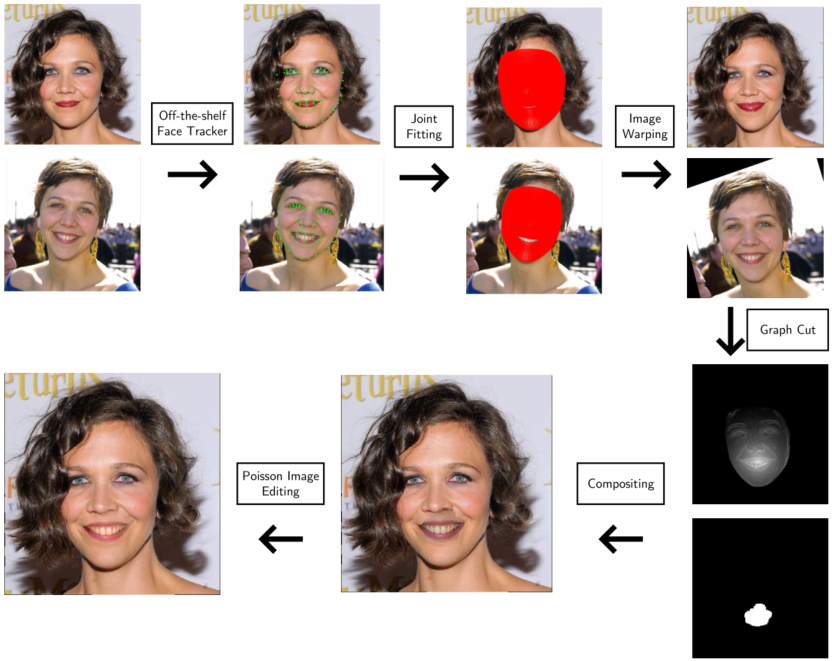
\includegraphics[width=\textwidth]{./img/expression-flow-pipeline}
\caption{Step 1: use the off-the-shelf face tracker to get the 2D face landmarks. \\
Step 2: Perform joint face fitting on the two face images. \\
Step 3: Perform image warping to align the two images for later image compositing. \\
Step 4: Generate prior map and perform graph cut to find the best seam. \\
Step 5: Sometimes there will be visible artifact on the border, we do one step of Poisson image edting on the composited image.}
\end{figure}

\subsection{Joint fitting of the model}
In some scenerios where we want to fit models for the same person that appeared in multiple images at the same time. We will need to fit the same identity weights $\mathbf{w}^{\text{id}}$ and fit the expression weights $\mathbf{w}^{\text{expr}}$ for different images. We adapt the previous algorithm as follows.

\subsection{Finding the best seam}
We can formulate this into a graph cut problem. In a graph cut framework. We first specify the data cost 
$$C(p) = \alpha \exp(-\frac{D_s(p)}{\sigma_d}) + (1 - \alpha) \left(1 - \exp(-\frac{||\nabla S(p)||}{\sigma_s})\right)$$
where $D_s(p)$ is the spatial distance from $p$ to the nearest pixel selected by the user, $||\nabla S(p)||$ is the gradient magnitude at $p$, and $\sigma_d$, $\sigma_s$ and $\alpha$ are parameters controlling the shape and weight of each term. $L(p)$ is the label of $p$. The data penalty in the graph cuts formulation is then defined as $C_d(p, L(p)) = 1 - C(p)$ is $L(p) = 1$(inside the crop region), and $C_d(p, L(p)) = C(p)$ if $L(p) = 0$(outside the crop region). 

Then we specify the smooth cost in the "match gradient" formulation for setting the neighborhood penalty $C_i(p, q, L(p), L(q))$ as:
$$||\nabla S_{L(p)}(p) - \nabla S_{L(p)}(p)|| + ||\nabla S_{L(p)}(q) - \nabla S_{L(q)}(q)||$$
This formulation encourages the cut to happen at the place where the difference of the gradients is small.


\subsection{Poisson Image Editing}
Here we introduce poisson image editing as a technique to remove visual seams. Visual seams occur because of the color mismatch between the two images. In poisson image editing we fix the colors of the boundary (taken from the background image) and provides a vector field that defines the structure of the image to be copied (taken from the foreground). The result image is generated by minimizing the squared error terms between the gradient of the result image and the guidance vector field.

The basic idea is to preserve the laplacian of the image while keep the boundary fixed.
$$\int_\Omega ||\Delta(\mathbf{x}_{1} - \hat{\mathbf{x}})||^2 \; d\mathbf{A} \quad \text{subject to } \hat{\mathbf{x}}^{\text{boundary}} = \mathbf{x}^{\text{boundary}}_2$$
Where the $\hat{\mathbf{x}}$ is the pixel value of inner part to be determined, $\mathbf{x}_1$ is the foreground image, $\mathbf{x}_2$ is the background image. 


\subsection{Results}
\begin{figure}[H]
    \centering
    \subfloat[]{\includegraphics[width=0.33\textwidth]{./img/flow2/img1}}
    \hfill
    \subfloat[]{\includegraphics[width=0.33\textwidth]{./img/flow2/img2}}
    \hfill
    \subfloat[]{\includegraphics[width=0.33\textwidth]{./img/flow2/blend_img}}
\end{figure}

\begin{figure}[H]
    \centering
    \subfloat[]{\includegraphics[width=0.33\textwidth]{./img/flow3/img1}}
    \hfill
    \subfloat[]{\includegraphics[width=0.33\textwidth]{./img/flow3/img2}}
    \hfill
    \subfloat[]{\includegraphics[width=0.33\textwidth]{./img/flow3/blend_img}}
\end{figure}

Here for each triple of images, we use the first image as the background image, the second as foreground image. Using the techniques described above, we get the third image as the result.

\section{Application 2: Face image editing using a 3D face model}
Intelligent manipulation of human facial images, such as expression editing is a hot topic in computer graphics. Here we introduce a system where inputting an image of a human face, the users can manipulate by moving the handle defined on the face mesh.

\subsection{Pipeline}
The pipeline is as follows:
\begin{enumerate}
\item Fit a face model to the image.
\item Manipulate the face model using laplacian mesh editing techniques.
\item Warp the original image according to the deformation field induced by the deformation of the underlying face model using the as-rigid-as-possible techniques.
\end{enumerate}

\subsection{Laplacian Mesh Editing}
To enable easy manipulation of the face mesh, we use the techniques called laplacian mesh editing.
Laplacian operator measures the flatness of the mesh:
$$\Delta f(\mathbf{x}) = \lim_{|B(\mathbf{x})| \rightarrow 0} \frac{1}{|B(\mathbf{x}))|} \int_{B(\mathbf{x})} f(\mathbf{z}) \;d\mathbf{z} - f(\mathbf{x})$$
Where $B(\mathbf{x})$ is an infinitesimal region around $\mathbf{x}$.
We want to the difference of mesh before and after deformation be small.  
\begin{align*}
\int_\Omega ||\Delta(\mathbf{x} - \hat{\mathbf{x}})||^2 \; d\mathbf{A} & \approx \text{tr}( \mathbf{D}^\top \mathbf{L}^\top \mathbf{M}^{-\top} \mathbf{M} \mathbf{M}^{-1} \mathbf{L}\mathbf{D})\\
&= \text{tr}(  \mathbf{D}^\top \underbrace{\mathbf{L}^\top \mathbf{M}^{-1} \mathbf{L}}_{\Q} \mathbf{D})
\end{align*}
where $\mathbf{D}, \mathbf{L}, \mathbf{M}$ is the difference of mesh, laplacian and the mass matrix respectively. 
$$
\min_{\D_\text{u}}
\tr \left((\D_\text{u}^\top \ \D_\text{h}^\top)
\left(\begin{array}{cc}
\Q_\text{u,u} & \Q_\text{u,h} \\
\Q_\text{h,u} & \Q_\text{h,h} 
\end{array}\right)
\left(\begin{array}{c}
  \D_\text{u} \\
  \D_\text{h}
\end{array}
\right)\right)
$$
$$
\min_{\D_\text{u}}
\tr\left(\D_\text{u}^\top \Q_\text{u,u} \D_\text{u} +
2 \D_\text{u}^\top \Q_\text{u,h} \D_\text{h} + 
\underbrace{\D_\text{h}^\top \Q_\text{h,h}
\D_\text{h}}_\text{constant}\right)
$$
$$
\min_{\D_\text{u}} 
\tr\left(
\D_\text{u}^\top \Q_\text{u,u} \D_\text{u} +
2 \D_\text{u}^\top \Q_\text{u,h} \D_\text{h})
\right)
$$
Set the gradient to zero
$$2 \Q_\text{u,u} \D_\text{u} + 2 \Q_\text{u,h} \D_\text{h} = 0 \rightarrow \D_\text{u} = \Q_\text{u,u}^{-1} \Q_\text{u,h} \D_\text{h}$$
Minimization w.r.t to the unconstrained points gives us the solution.

\subsection{As-rigid-as-possible image manipulation}
We can perform the laplacian mesh editing to get the deformed 3D model. Now we want to manipulate the image which corresponds to the model deformation. To achieve this, we first construct a mesh on the image and project the vertices of the 3D model to guide the deformation of the image using the as-rigid-as-possible shape manipulation techniques\cite{igarashi2005rigid}.

\subsection{Results}
Here we show three results using the techniques described above.
\begin{figure}[H]
  \includegraphics[width=\textwidth]{./img/laplacian.pdf}
\end{figure}
These three results shows that the system can perform 3D aware face image manipulation without artifact.

\section{Code structure}
The code structure is as follows:
\begin{itemize}
\item \texttt{src/arap} contains the code of implementation of \cite{igarashi2005rigid}.
\item \texttt{src/fitmodel} contains the code of implementation of single image fitting and joint shape fitting, described in \cite{yang2011expression}.
\item \texttt{src/seamless\_composite} contains the code of implementation of seamless compositing of two images, described in \cite{agarwala2004interactive}.
\item \texttt{src/poisson\_blend} contains the code of implementation of poisson image editing, described in \cite{perez2003poisson}.
\item \texttt{src/laplacian} contains the code of laplacian mesh editing\cite{sorkine2004laplacian}. We refer to this repository for implementation of GUI.\footnote{https://github.com/alecjacobson/geometry-processing-deformation} 
\item \texttt{src/demo} contains the code of two demos built on top of the techniques described above.
\end{itemize}
\section{Summary}
In this project, we have implemented the following:
\begin{itemize}
\item Single/Joint Face fitting \cite{yang2011expression}
\item Laplacian Surface Editing \cite{sorkine2004laplacian}
\item Poisson Image Editing \cite{perez2003poisson}
\item Formulate our problem into graph cut\cite{yang2011expression} and solve it using GCO library \cite{boykov2004experimental}
\item ARAP shape manipulation \cite{igarashi2005rigid}
\item \textbf{Combine the above all together}
\end{itemize}
Based on these techniques we have implemented, we build two interesting applications. The first one is facial component transfer and the second one is easy face editing.

 

    
\bibliographystyle{apalike}
\bibliography{ref}
 
\end{document}